The classes SOM, RNA et NEURON are a minimalist adaptation of the code source \textsl{Neuromuse}\footnote{\href{https://github.com/FredVoisin/neuromuse}{\texttt{\scriptsize https://github.com/FredVoisin/neuromuse}}} which aims to allow a flexibility to manage parameters. In short, it is question to initiate a Self Organizing Map in terms of learning and activation. 

\bigskip

The Self Organizing Map is a concept formalised and modeled in 1980 by Teuvo Kohonen. It is a model of an artificial neural network working by competition for a set of given stimuli. This allows to create a topology for classification, interpolation or displaying multidimensional data.

\bigskip

\begin{displayquote}
The map consists of a regular grid of processing units, `neurons'. A model of some multidimensional observation, eventually a vector consisting of features, is associated with each unit. The map attempts to represent all the available observations with optimal accuracy using a restricted set of models. At the same time the models become ordered on the grid so that similar models are close to each other and dissimilar models far from each other. 

\smallskip 

Fitting of the model vectors is usually carried out by a sequential regression process, where $t = 1,2,...$ is the step index. For each sample $x(t)$, first the winner index $c$ (best match) is identified by the condition:

$$\forall i, || x(t) - m_c(t) || \leq || x(t) - m_i(t) ||$$

After that, all model vectors or a subset of them that belong to nodes centered around node $c = c(x)$ are updated as:

$$m_i(t + 1) = m_i(t) + h_{c(x),i}(x(t) - m_i(t))$$

Here $h_{c(x),i}$ is the `neighborhood function', a decreasing function of the distance between the $i$th and $c$th nodes on the map grid. This regression is usually reiterated over the available samples.\footnote{\href{http://www.cis.hut.fi/research/som-research/som.shtml}{\texttt{\scriptsize http://www.cis.hut.fi/research/som-research/som.shtml}}}
\end{displayquote}

%\bigskip
%
%First of all, here are some guidelines of how to use functions defined in the user file as parameters in N3 context. These functions require two or three arguments and optionally a list of additional argument(s). To set a function, a list is required with as first argument the function itself, and optionally the remaining option(s) belonging to the function. 

\bigskip

Here are some guidelines about the available parameters in N3.

\bigskip
%\newpage
Functions required for the class SOM as slots:

\begin{itemize}
\item The map function -- slot \texttt{carte} -- to initiate the neurons of the SOM.
\item The neighborhood function -- slot \texttt{voisinage} -- which defines the type of influence that the winning neuron will have on its neighbors allowing to update the network during the learning process (usually a gaussian or a `mexican hat' function).
\item The proximity function to define the type of relationship %(always in terms of distance, although this may be different, for example in terms of standard deviation) 
between two neurons -- slot \texttt{distance-in} --  
%involving the positions or the outputs, 
or between a set of stimuli and its response -- slot \texttt{distance-out} -- when the SOM is activated in order to set and to minimalize errors for the winning neuron selection.
\end{itemize}

\bigskip

The SOM initiation is done either with the defmethod \texttt{init-som} or simply with the N3 function \glspl{create-mlt} with as arguments the name of the SOM, the number of stimuli and the number of neurons in the map.

\smallskip

The activation consists to compute for each neuron the error defined by $|| x(t) - m_i(t) ||$. 

\smallskip

Note that the data input has to be adjusted such as each component has a value between 0 and 1 in order to match the range of the output as weight values during initialisation.

\bigskip

The learning step refers to the class RNA according to the slots:

\begin{itemize}
\item \texttt{learning-rate} as the maximum correction value applied to the winning neuron;
\item \texttt{radius} as influence of the winning neuron on its neighbors. 
\end{itemize}

\begin{figure}[htbp]
\begin{center}
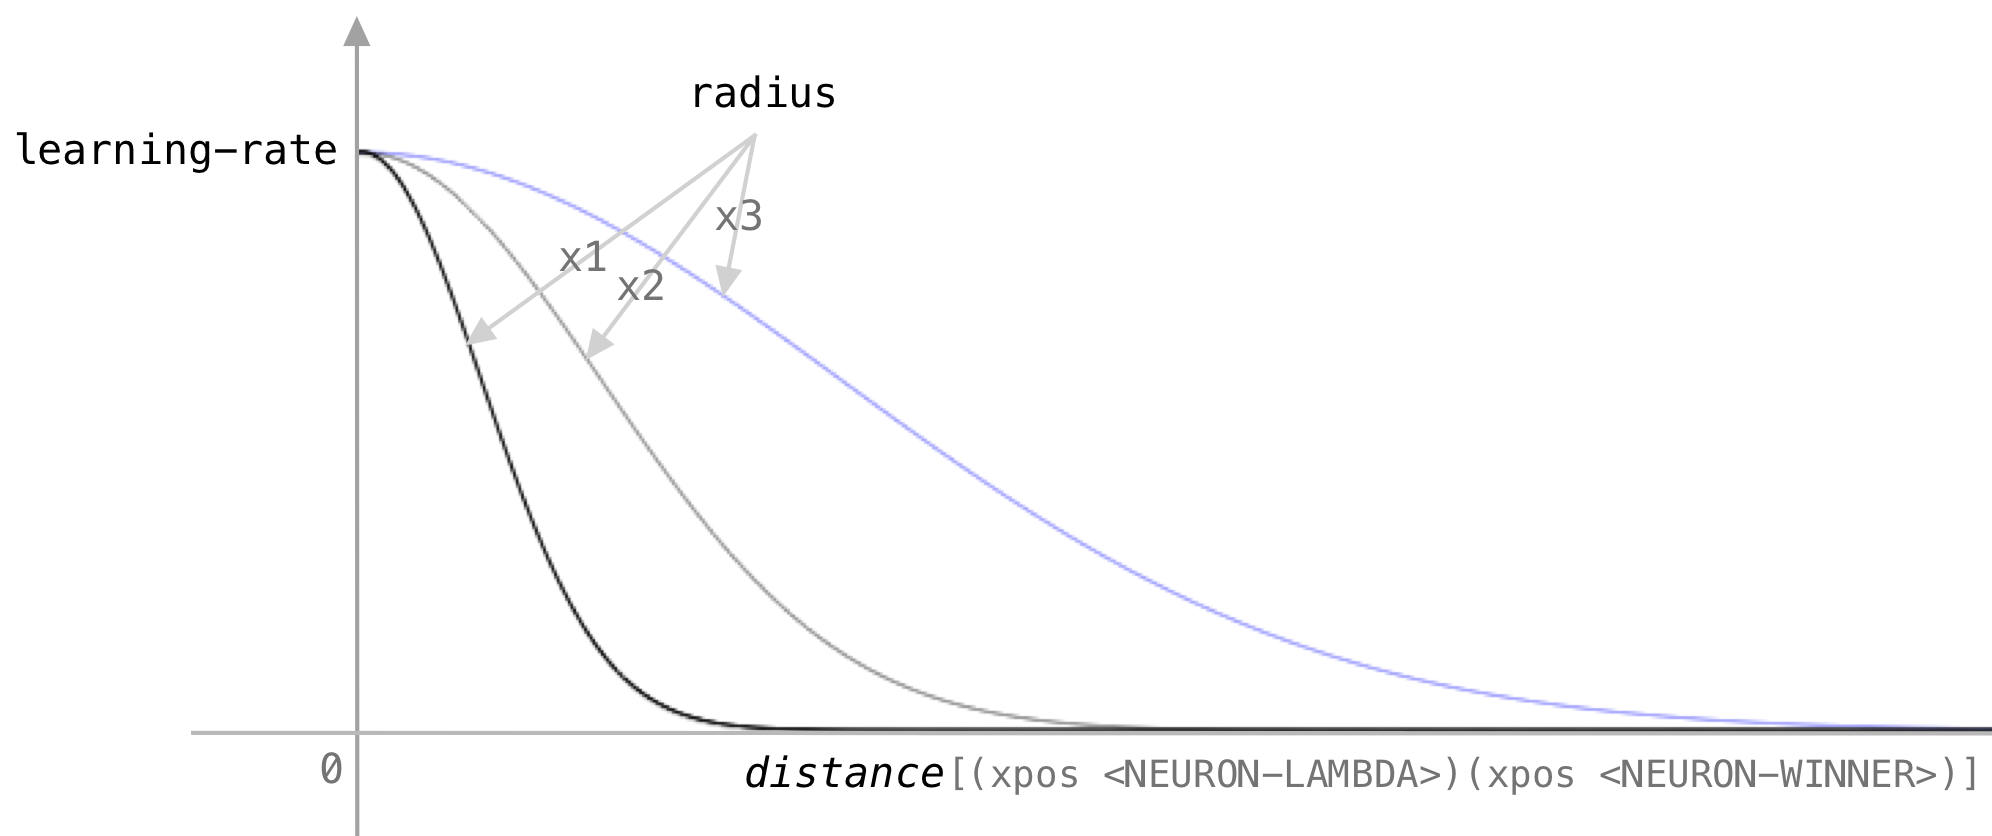
\includegraphics[width=\columnwidth]{2311}
\caption{The neighborhood function \glspl{gauss} with its parameters. %The `half' Bell shape is proportional to the radius ...
}
\label{fig:gs}
\end{center}
\end{figure}

See Table \ref{table:bf} concerning functions which can be set in a SOM as described previously. 

See also Table \ref{table:class} on page \pageref{table:class} for all parameters and properties.

\begin{table}[htp]
\caption{\label{table:bf}The package N3 provides some basic functions about SOM.}
\begin{center}
\begin{tabular}{| p{3cm} | p{5.5cm}}
Mapping & \glspl{quadrare}, \glspl{rnd-map} \\ 
Proximity & \glspl{euclidean} \\  
Neighborhood & \glspl{gauss}, \glspl{fn-mex} \\   
Decreasing & \glspl{exp-decay} 
\end{tabular}
\end{center}
\end{table}%